\clearpage
\chapter*{LAMPIRAN}
\phantomsection
\addcontentsline{toc}{chapter}{LAMPIRAN}
\setcounter{table}{0}
\renewcommand{\thetable}{L.\arabic{table}}
\setcounter{figure}{0}
\renewcommand{\thefigure}{L.\arabic{figure}}
% Lampiran adalah ringkasan yang dapat ditelusuri ke berkas proyek. Data hasil tidak
% disalin atau dibuat ulang di sini. Instrumen UAT belum diisi oleh peserta.

\section*{Lampiran A. Basis Pengetahuan Resep dan Asumsi}
\phantomsection
\addcontentsline{toc}{section}{Lampiran A. Basis Pengetahuan Resep dan Asumsi}

Arahan pembimbing menjadi sumber tujuh kelompok resep pada Tabel~\ref{tab:lampiran-resep}. Nama, langkah, dan angka asli disimpan bersama penanda \texttt{source=pdf\_arahan} di \path{app/backend/app/seed/recipes.json} dan SOP terkait. Ringkasan ini dipakai untuk mengaudit hubungan antara arahan, resep digital, dan uji kalkulator; berkas JSON merupakan daftar terperinci yang dijalankan aplikasi.

\begin{table}[htbp]
\centering
\caption{Ringkasan Angka Resep dari Arahan Pembimbing}
\label{tab:lampiran-resep}
\small
\begin{tabular}{>{\RaggedRight\arraybackslash}p{.26\textwidth}>{\RaggedRight\arraybackslash}p{.61\textwidth}}
\toprule
Resep & Fakta dalam arahan \\
\midrule
Caffè Latte panas & Satu \textit{shot} espreso ganda, susu segar dengan \textit{microfoam} tipis sekitar 1~cm, cangkir 200--250~ml; susu 60--65~$^\circ$C. \\
Cappuccino panas & Satu \textit{shot} espreso, susu panas dengan busa tebal sekitar 1,5--2~cm; cangkir 150--180~ml. \\
Ice Brown Sugar Shaken Espresso & Dua \textit{shot} espreso, 20~ml sirup gula aren, es secukupnya, dan susu segar sebagai pengisi. \\
Americano/Long Black & Dua \textit{shot} espreso dan air mineral atau es; Long Black menuangkan air lebih dulu, Americano espreso lebih dulu. \\
V60/\textit{Pour Over} & Kopi 15~g dan air 225~ml (1:15), air 90--92~$^\circ$C. \textit{Bloom} 45~ml selama 30--45 detik, target 130~ml pada menit 1:00 dan 225~ml pada menit 1:30; selesai 2:30--3:00. \\
Iced Matchagato/Matcha Latte Creamy & Matcha 5~g, air hangat 15~ml, sirup sederhana 15~ml, susu segar 150~ml, dan es; matcha dilarutkan lebih dulu. \\
Signature Pandan Latte & Satu \textit{shot} espreso, ekstrak pandan 20~ml, susu segar 150~ml, dan es; sirup pandan berada di dasar, espreso di atas. \\
\bottomrule
\end{tabular}
\end{table}

Angka yang tidak berasal dari arahan dicatat di \path{app/backend/app/seed/ASSUMPTIONS.md} dengan kode A01--A25. Tabel~\ref{tab:lampiran-asumsi} menyajikan asumsi yang paling berpengaruh pada hasil. Seluruh stok awal, waktu pasok, ukuran kemasan, dan jumlah pesan adalah data contoh; pembaca dapat menggantinya dengan hasil pengamatan kedai tanpa mengubah fakta resep yang berasal dari arahan.

\begin{table}[htbp]
\centering
\caption{Asumsi Utama Implementasi dan Dampaknya}
\label{tab:lampiran-asumsi}
\begin{tabular}{lp{.34\textwidth}p{.39\textwidth}}
\toprule
Kode & Isi & Dampak \\
\midrule
A01--A03 & Arti \textit{shot} ganda dan parameter espreso tambahan. & Kebutuhan biji dan volume komponen. \\
A04--A06 & Ukuran cangkir, ekspansi susu, massa jenis es. & Sisa ruang dan takaran pengisi. \\
A09--A10 & Ketelitian takar dan batas kurang isi. & Pembulatan dan peringatan kalkulator. \\
A11--A14 & Dosis V60 dan batas kemanisan. & Variasi pesanan yang dapat diproses. \\
A16, A24 & Stok, \textit{lead time}, kemasan, parameter simulasi. & Status serta kuantitas \textit{restock}. \\
A25 & Batas kewajaran masukan seduh. & Input yang diterima sistem pakar. \\
\bottomrule
\end{tabular}
\end{table}

\section*{Lampiran B. Pemetaan Produk dan Aturan AI}
\phantomsection
\addcontentsline{toc}{section}{Lampiran B. Pemetaan Produk dan Aturan AI}

Pemetaan lengkap antara produk IBM/Maven dan resep disimpan sebagai \path{app/backend/app/seed/product_recipe_map.json}; penjelasan asumsi ukuran dan proksi berada pada \path{ASSUMPTIONS.md}. Produk Latte dipetakan ke Caffè Latte, Cappuccino ke resep Cappuccino, minuman espreso ke subresep espreso, dan seduhan filter ke V60. Cokelat panas, chai, serta teh menggunakan resep tambahan yang nilainya dinyatakan asumsi. Roti dan barang kemasan tidak diuraikan ke bahan resep. Nama produk yang dipakai untuk pasangan menu dinormalisasi ke kunci tanpa ukuran, sedangkan pemetaan ke resep dipakai saat ramalan penjualan diubah menjadi kebutuhan bahan.

Basis pengetahuan koreksi seduh tersimpan pada \path{app/backend/app/ai/kb/brew_rules.json}. Setiap aturan memuat kondisi, fakta yang disimpulkan, prioritas, saran, dan sumber. Jejak aturan dikembalikan kepada pengguna agar diagnosis dapat diperiksa. Hasil evaluasi E4 menunjukkan mengapa jejak itu diperlukan: arah kekuatan hanya cocok dengan sebagian penilaian konsumen, dan preferensi kesukaan tidak sama dengan berada di kotak teknis \textit{Golden Cup}. Daftar aturan lengkap lebih tepat dibaca dari berkas JSON yang digunakan mesin daripada ditranskripsi ulang ke naskah.

\section*{Lampiran C. Ringkasan Kasus Pengujian Otomatis}
\phantomsection
\addcontentsline{toc}{section}{Lampiran C. Ringkasan Kasus Pengujian Otomatis}

Kasus \textit{black-box} antarmuka terperinci berada di \path{app/results/tests/blackbox_cases.csv}. Berkas itu memuat identitas, langkah, hasil yang diharapkan, hasil aktual, dan status otomatis. Tabel~\ref{tab:lampiran-kasus} memudahkan pencarian kelompok kasus; bukti tangkapan layar berada di \path{app/results/screenshots/blackbox}. Jumlah lulus pada Bab~\ref{bab:hasil} mengacu pada berkas yang diregenerasi setelah perubahan kode terakhir.

\begin{table}[htbp]
\centering
\caption{Cakupan Kasus \textit{Black-Box} Antarmuka}
\label{tab:lampiran-kasus}
\begin{tabular}{lp{.69\textwidth}}
\toprule
ID & Cakupan \\
\midrule
BB-01--BB-04 & Masuk tiga peran, navigasi berizin, dan kata sandi keliru. \\
BB-05--BB-08 & Katalog dan detail resep, ukuran latte, kalkulator V60. \\
BB-09--BB-10 & Pencatatan produksi, pengurangan stok, penerimaan dan opname. \\
BB-11--BB-14 & Checklist SOP, panduan V60, timer espreso, diagnosis seduh. \\
BB-15--BB-18 & \textit{Restock}, prakiraan, pasangan menu, dan metrik evaluasi AI. \\
BB-19--BB-22 & Akun pengguna, data/model, keluar, dan navigasi ponsel. \\
BB-23--BB-26 & Perubahan resep/SOP, detail V60, dan ringkasan beranda. \\
BB-27 & Asisten AI menampilkan jawaban V60 yang relevan dan rujukan resep/SOP. \\
BB-28 & Animasi Panduan Seduh menampilkan tindakan, waktu, dan target sesuai tahap resep aktif. \\
BB-29 & Tautan saran pasangan menu membuka Panduan Seduh pada resep yang cocok. \\
\bottomrule
\end{tabular}
\end{table}

\section*{Lampiran D. Instrumen Uji Penerimaan Pengguna}
\phantomsection
\addcontentsline{toc}{section}{Lampiran D. Instrumen Uji Penerimaan Pengguna}

Instrumen ini disiapkan untuk sesi barista dan pengelola kedai; belum ada responden atau skor yang diisi. Sebelum sesi, peneliti mencatat kode peserta tanpa nama di lembar analisis, peran pekerjaan, pengalaman meracik kopi, perangkat, tanggal, dan versi aplikasi. Peserta diberi akun sesuai peran dan diminta mengerjakan tugas tanpa demonstrasi penyelesaian. Peneliti mencatat keberhasilan, waktu, bantuan yang diberikan, dan masalah yang teramati. Kata sandi demo diganti sebelum pengujian di lingkungan bersama.

\begin{table}[H]
\centering
\caption{Tugas UAT dan Kriteria Keberhasilan}
\label{tab:lampiran-uat}
\small
\begin{tabular}{l>{\RaggedRight\arraybackslash}p{.49\textwidth}>{\RaggedRight\arraybackslash}p{.32\textwidth}}
\toprule
ID & Tugas peserta & Kriteria keberhasilan \\
\midrule
U1 & Temukan resep Caffè Latte dan jelaskan takaran serta suhu susu. & Halaman resep tepat; informasi standar ditemukan. \\
U2 & Hitung tiga Caffè Latte ukuran besar dengan tambahan satu \textit{shot}. & Takaran per cangkir, total, dan peringatan terbaca. \\
U3 & Hitung V60 dosis 20~g dan temukan target tuang bertahap. & Air 300~ml dan target 60/173,3/300~ml ditemukan. \\
U4 & Jalankan panduan seduh dan timer sampai langkah berikutnya. & Timer serta target langkah dipakai dengan benar. \\
U5 & Catat satu produksi dan periksa perubahan stok bahan. & Log produksi dan mutasi stok yang sesuai ditemukan. \\
U6 & Kerjakan checklist pembukaan bar. & Langkah kritis ditandai dan status selesai tersimpan. \\
U7 & Temukan bahan yang perlu dipesan ulang dan jelaskan dasar sarannya. & Status, jumlah pesan, dan label data contoh dipahami. \\
U8 & Masukkan gejala seduhan dan baca alasan diagnosis. & Saran dan aturan yang terpenuhi ditemukan. \\
U9 & Ajukan pertanyaan resep kepada asisten AI lokal dan buka sumber jawabannya. & Jawaban, mode, dan rujukan yang relevan terbaca. \\
U10 & Pilih saran pasangan menu yang memiliki resep aktif, buka panduannya, lalu ikuti ilustrasi tahap seduh. & Tautan menuju resep benar; tindakan, waktu, dan target tahap dijelaskan sesuai panduan. \\
\bottomrule
\end{tabular}
\end{table}

Sesudah tugas, peserta mengisi 10 pernyataan SUS berikut dengan skala 1 = sangat tidak setuju sampai 5 = sangat setuju. Redaksi Bahasa Indonesia ini disiapkan sebagai instrumen penelitian, sehingga pemahaman istilah perlu diperiksa pada sesi percontohan. Butir ganjil bersifat positif dan butir genap negatif sesuai pola SUS \citep*{brooke1996sus}.

\begin{table}[H]
\centering
\caption{Kuesioner \textit{System Usability Scale} yang Disiapkan}
\label{tab:lampiran-sus}
\begin{tabular}{r>{\RaggedRight\arraybackslash}p{.76\textwidth}}
\toprule
No. & Pernyataan \\
\midrule
1 & Saya merasa akan sering menggunakan aplikasi ini. \\
2 & Saya merasa aplikasi ini terlalu rumit untuk digunakan. \\
3 & Saya merasa aplikasi ini mudah digunakan. \\
4 & Saya merasa memerlukan bantuan orang yang memahami teknis untuk menggunakan aplikasi ini. \\
5 & Saya merasa fungsi-fungsi dalam aplikasi ini terintegrasi dengan baik. \\
6 & Saya merasa terdapat terlalu banyak hal yang tidak konsisten dalam aplikasi ini. \\
7 & Saya membayangkan kebanyakan orang akan cepat belajar menggunakan aplikasi ini. \\
8 & Saya merasa aplikasi ini sangat merepotkan untuk digunakan. \\
9 & Saya merasa yakin ketika menggunakan aplikasi ini. \\
10 & Saya perlu mempelajari banyak hal sebelum dapat menggunakan aplikasi ini. \\
\bottomrule
\end{tabular}
\end{table}

Skor tiap butir ganjil dihitung sebagai jawaban dikurangi satu; butir genap sebagai lima dikurangi jawaban. Jumlah kontribusi sepuluh butir dikalikan 2,5 untuk memperoleh skor 0--100 per peserta. Rerata baru dihitung setelah jawaban nyata tersedia, disertai jumlah peserta dan sebarannya. Skor tidak boleh diisi dari perkiraan peneliti atau hasil pengujian otomatis.

\section*{Lampiran E. Reproduksi Hasil}
\phantomsection
\addcontentsline{toc}{section}{Lampiran E. Reproduksi Hasil}

Dataset yang diperlukan ditempatkan sesuai \path{dataset/raw/*/DATASHEET.md}. Dari folder \path{app}, instalasi dilakukan dengan \path{setup.bat}, lalu aplikasi dijalankan dengan \path{run.bat}. Untuk mengulang evaluasi, jalankan perintah berikut dari \path{app/backend} menggunakan lingkungan Python yang dibuat \path{setup.bat}. Setiap skrip menulis parameter, hash data, dan hasil baru ke \path{app/results}; keluaran lama tidak perlu disalin manual.

\begin{verbatim}
.venv\Scripts\python.exe scripts\evaluate_scaling.py
.venv\Scripts\python.exe scripts\evaluate_pairing.py
.venv\Scripts\python.exe scripts\evaluate_forecasting.py
.venv\Scripts\python.exe scripts\evaluate_restock.py
.venv\Scripts\python.exe scripts\evaluate_pairing_external.py
.venv\Scripts\python.exe scripts\evaluate_forecasting_external.py
.venv\Scripts\python.exe scripts\evaluate_restock_external.py
.venv\Scripts\python.exe scripts\validate_expert_system.py
.venv\Scripts\python.exe scripts\validate_scaling_starbucks.py
.venv\Scripts\python.exe scripts\check_external_results.py
.venv\Scripts\python.exe scripts\evaluate_assistant.py
.venv\Scripts\python.exe -m pytest -q
\end{verbatim}

Evaluasi asisten memerlukan Ollama dan kedua model Gemma 4 yang disebut pada Bab~\ref{bab:hasil}; skrip menjalankan tujuh varian pada 60 butir dan menyimpan jawaban beserta skor. Hasil yang dilaporkan menggabungkan 300 jawaban kondisi lama dengan 120 jawaban RAG dan alat setelah perbaikan router; prosesnya dapat diulang secara deterministik dari jawaban mentah yang disimpan dengan perintah berikut. Skrip penggabungan menolak hash tolok ukur atau basis data yang berbeda; skrip penilai ulang tidak memanggil model. Menjalankan evaluasi dari awal dapat menghasilkan jawaban berbeda karena perangkat dan runtime model dapat berubah.

\begin{verbatim}
.venv\Scripts\python.exe scripts\merge_assistant_eval.py
.venv\Scripts\python.exe scripts\rescore_assistant.py ^
  --input ..\results\assistant_eval_merged_raw.json ^
  --output-stem assistant_eval
\end{verbatim}

Tanda \texttt{\^{}} pada baris perintah di atas adalah penyambung baris Windows; kedua baris \texttt{rescore\_assistant.py} dapat pula ditulis dalam satu baris. Pengujian antarmuka dijalankan dari \path{app/frontend} dengan \texttt{npm run build}, \texttt{npm run test:e2e}, dan \texttt{npm run screenshots}. Pengukuran API memakai \path{scripts/measure_api_latency.py}; Lighthouse memakai \texttt{npm run lighthouse}. Waktu pengukuran latensi dan skor Lighthouse dapat berubah sesuai komputer serta beban saat pelaksanaan.

\section*{Lampiran F. Tampilan Panduan Seduh Beranimasi}
\phantomsection
\addcontentsline{toc}{section}{Lampiran F. Tampilan Panduan Seduh Beranimasi}

Gambar~\ref{fig:lampiran-animasi-v60} dan Gambar~\ref{fig:lampiran-animasi-espresso} memperlihatkan keadaan antarmuka ketika tahap resep ditampilkan. Gambar diam hanya mendokumentasikan satu posisi ilustrasi; gerak, jeda, dan pergantian tahap diperiksa melalui pengujian antarmuka BB-28. Gambar~\ref{fig:lampiran-pairing-panduan} memperlihatkan tautan panduan pada saran yang memiliki padanan resep aktif, sedangkan Gambar~\ref{fig:lampiran-pairing-mobile} menunjukkan tahap yang dibuka pada ponsel setelah tautan itu dipilih dalam BB-29. Gambar-gambar ini adalah bukti implementasi, bukan hasil pengukuran keberhasilan belajar pengguna.

\begin{figure}[htbp]
\centering
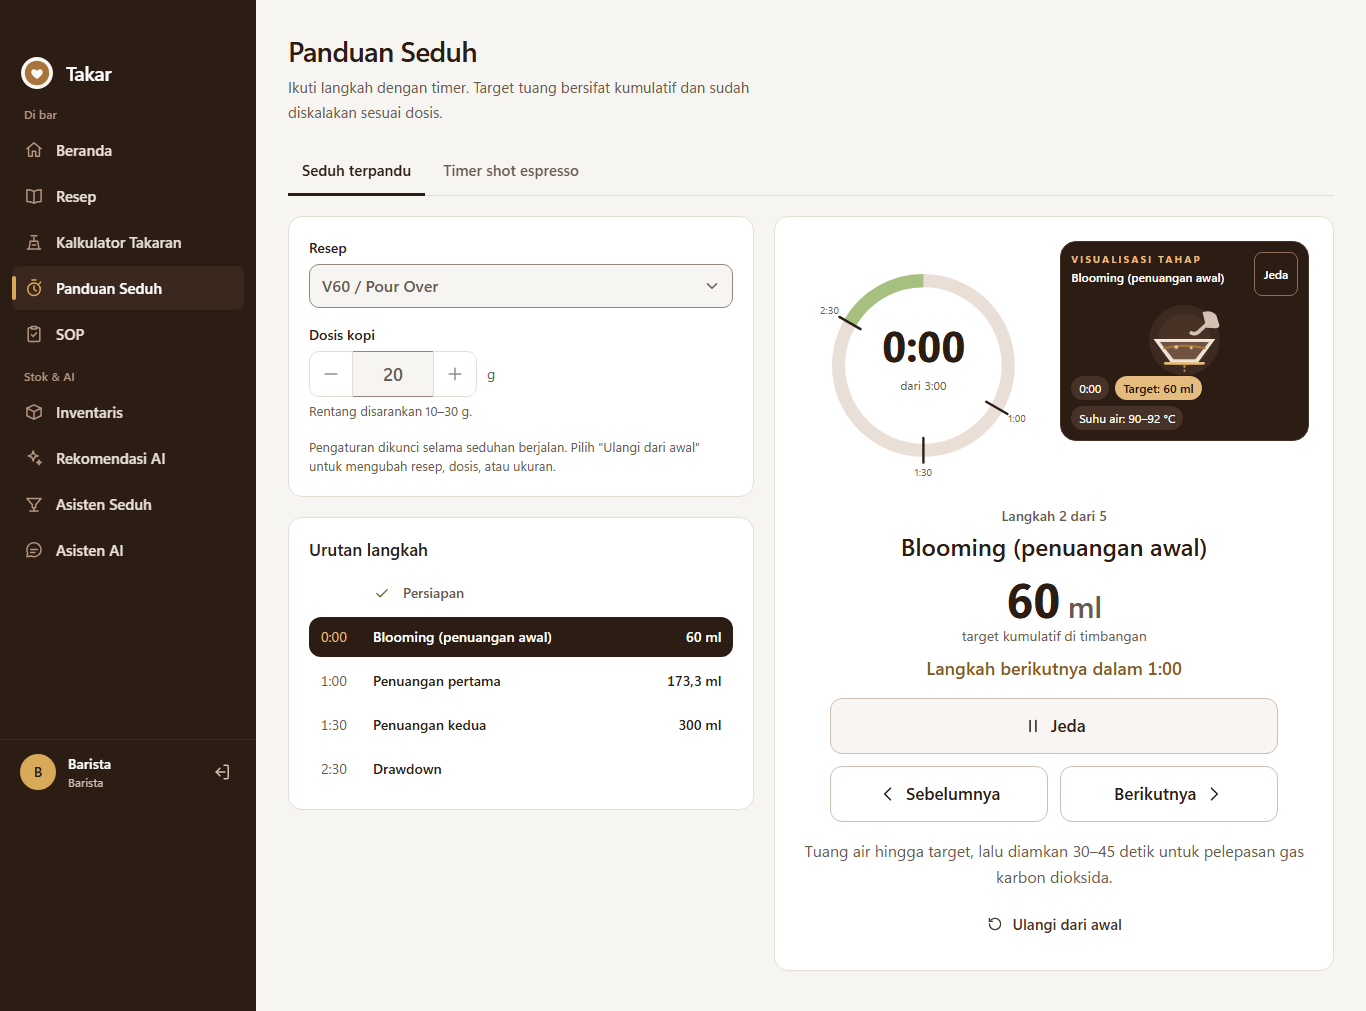
\includegraphics[width=.82\textwidth]{pic/results/screenshots/blackbox/BB-28-brew-animation.png}
\caption{Tahap \textit{blooming} V60 dosis 20~g dengan ilustrasi bergerak, timer aktif, dan target 60~ml}
\label{fig:lampiran-animasi-v60}
\end{figure}

\begin{figure}[htbp]
\centering
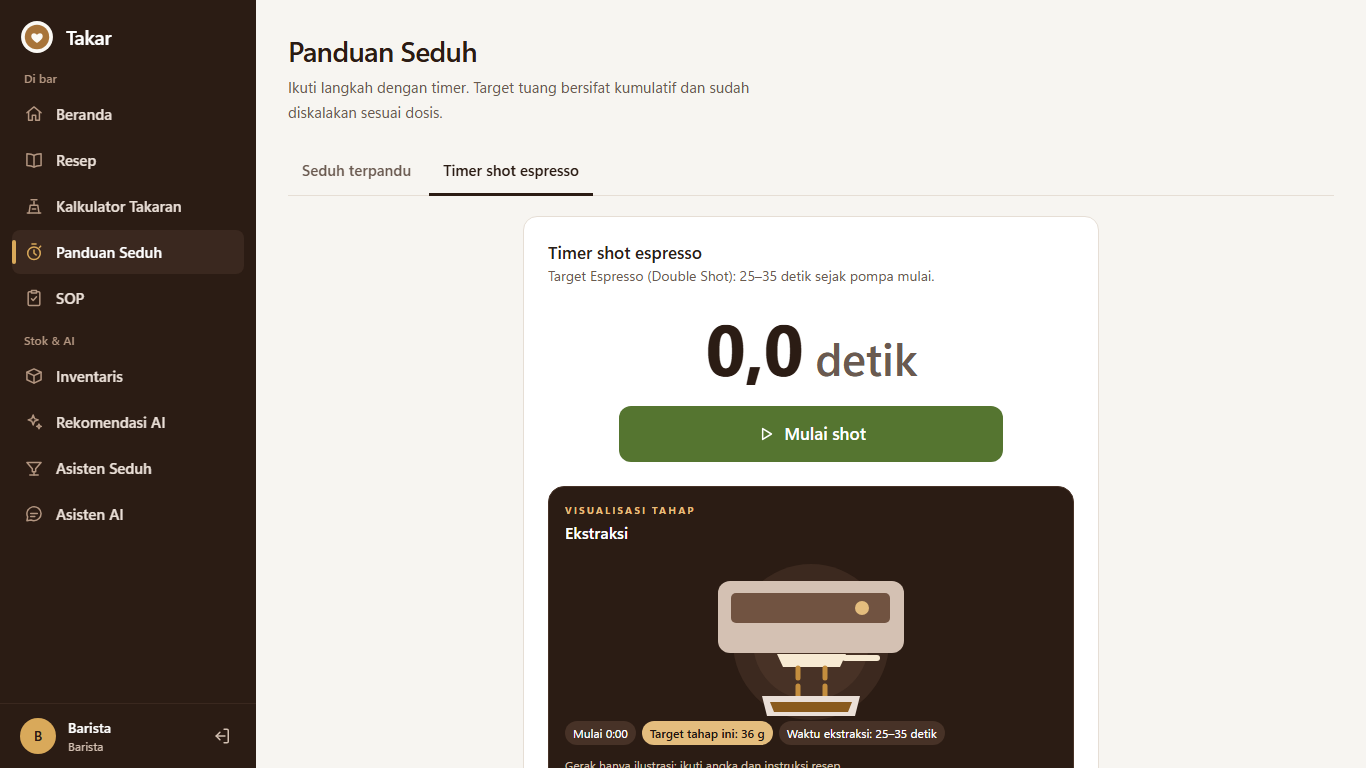
\includegraphics[width=.88\textwidth]{pic/results/screenshots/desktop/10-timer-shot-espresso.png}
\caption{Ilustrasi ekstraksi pada Timer Shot Espresso dengan target waktu dan hasil resep}
\label{fig:lampiran-animasi-espresso}
\end{figure}

\begin{figure}[htbp]
\centering
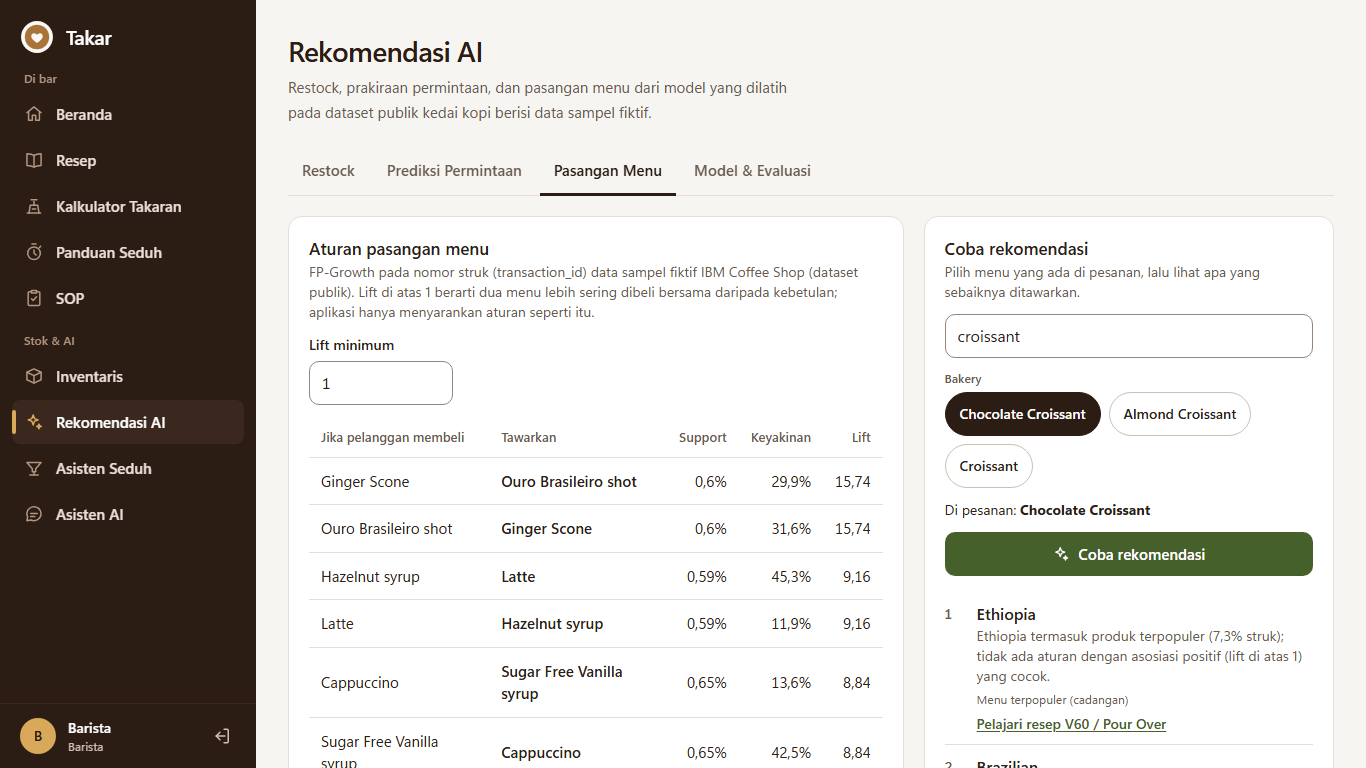
\includegraphics[width=.88\textwidth]{pic/results/screenshots/desktop/18-ai-pasangan-menu.png}
\caption{Tautan ``Pelajari resep V60 / Pour Over'' pada saran pasangan menu}
\label{fig:lampiran-pairing-panduan}
\end{figure}

\begin{figure}[htbp]
\centering
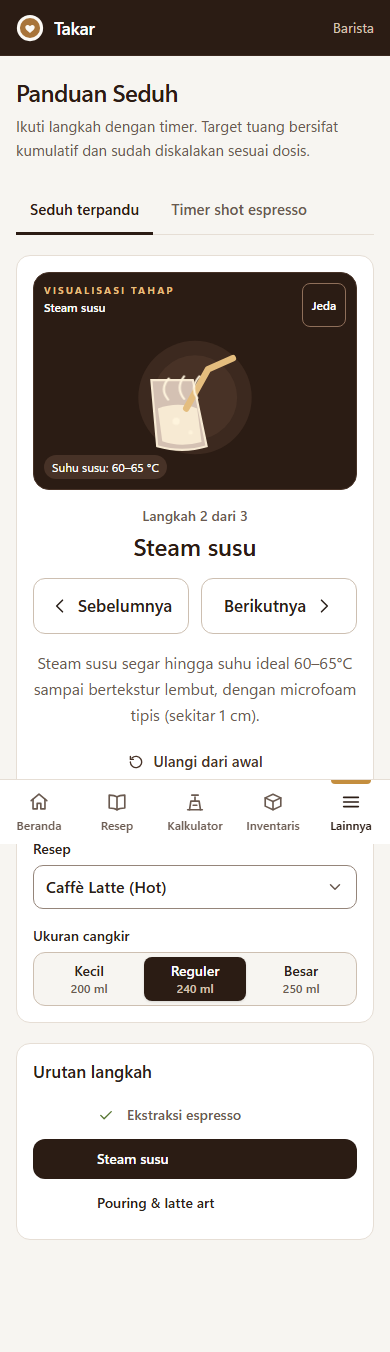
\includegraphics[width=.36\textwidth]{pic/results/screenshots/blackbox/BB-29-pairing-brew-link.png}
\caption{Tahap pengukusan susu Caffè Latte pada ponsel setelah panduan dibuka dari pasangan menu}
\label{fig:lampiran-pairing-mobile}
\end{figure}

\clearpage
\section*{Lampiran G. Contoh Jawaban Asisten dengan Sumber}
\phantomsection
\addcontentsline{toc}{section}{Lampiran G. Contoh Jawaban Asisten dengan Sumber}

Gambar~\ref{fig:lampiran-asisten} memperlihatkan jawaban asisten tentang prosedur V60 dalam BB-27, termasuk langkah dan rujukan yang dapat dibuka. Satu jawaban contoh tidak mewakili seluruh pertanyaan; hasil 60 butir untuk tiap varian dilaporkan pada Bab~\ref{bab:hasil} dan tersimpan di \path{app/results/assistant_eval.json}.

\begin{figure}[htbp]
\centering
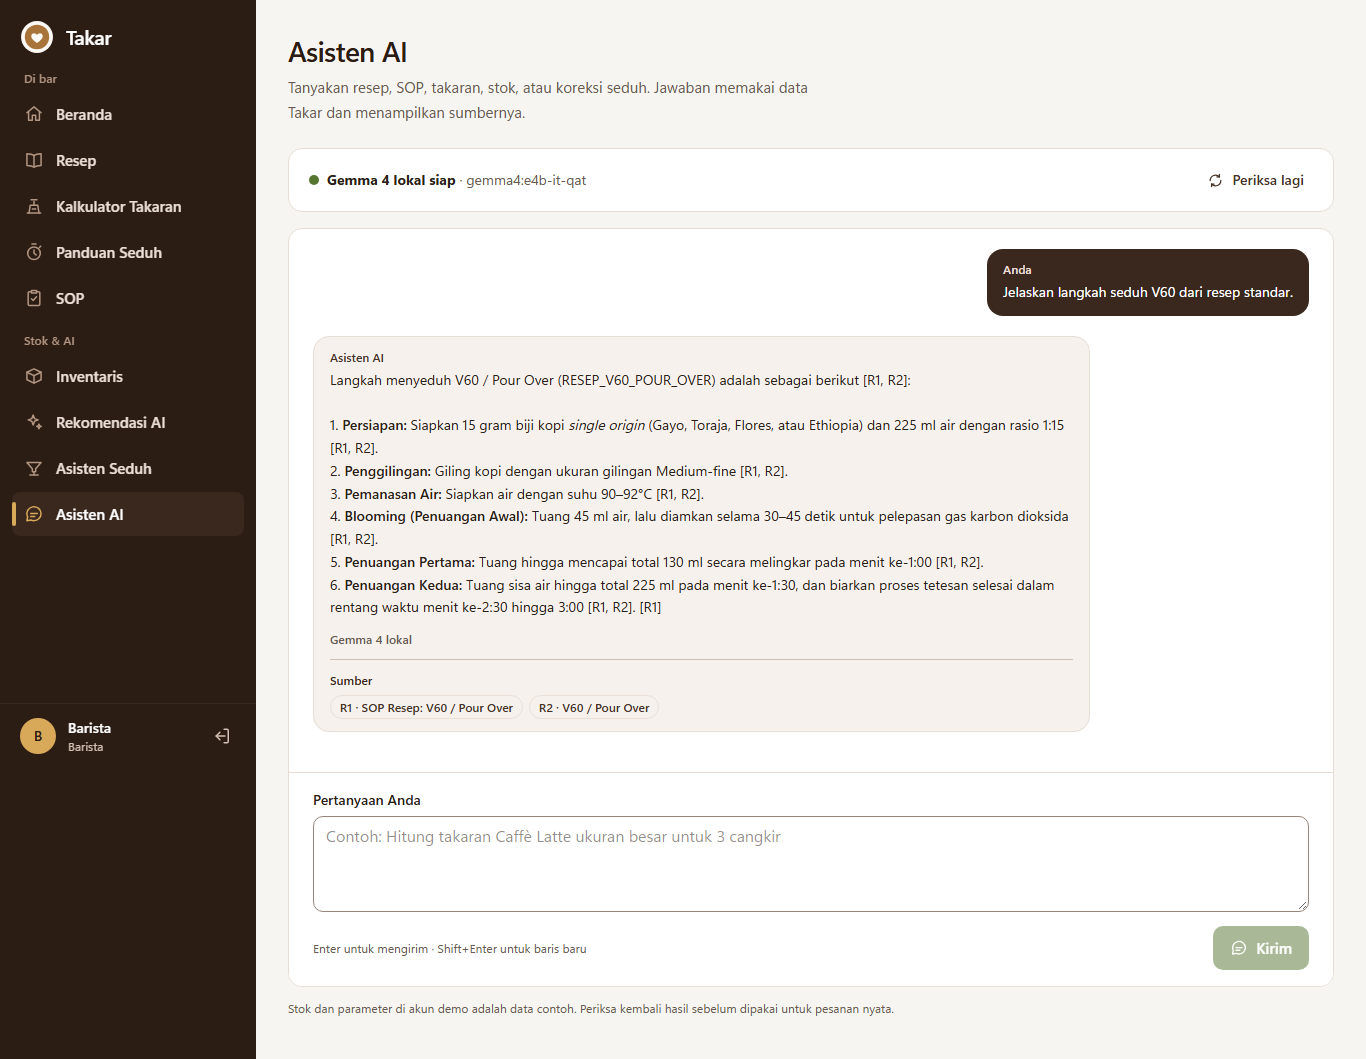
\includegraphics[width=.88\textwidth]{pic/results/screenshots/blackbox/BB-27-assistant-ai.png}
\caption{Jawaban Asisten AI tentang V60 dengan Rujukan Resep dan SOP}
\label{fig:lampiran-asisten}
\end{figure}
